\documentclass{standalone}
\usepackage{tikz}
\usepackage{ctex,siunitx,ninecolors}
\usepackage{tkz-euclide}
\usepackage{amsmath}
\usetikzlibrary{patterns, calc}
\usetikzlibrary {decorations.pathmorphing, decorations.pathreplacing, decorations.shapes,}
\begin{document}
\small
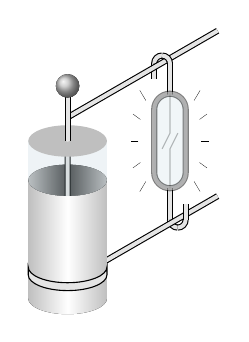
\begin{tikzpicture}[>=stealth]
  \fill[left color=lightgray,right color=lightgray,middle color=darkgray](0,-1.0)ellipse(0.5 and 0.2);
  \draw[double=lightgray!40,rounded corners,double distance=0.5mm]([yshift=-1.5mm]30:1.27)--++(0,-0.2);
  \draw[double=lightgray!40,rounded corners,double distance=0.5mm]([yshift=-1.5mm]30:1.27)arc(180:90:0.1) coordinate(A);
  \draw[double=lightgray!40,rounded corners,double distance=0.5mm](0,-0.2)--++(30:2.2);
  \draw[double=lightgray!40,rounded corners,double distance=0.5mm](A)arc(90:0:0.1)coordinate(C);
  \draw[double=lightgray!40,rounded corners,double distance=0.5mm](C)--++(0,-0.4);
  \draw[double=lightgray!40,rounded corners,double distance=0.5mm]([yshift=-18.5mm]30:1.5)--++(0,-0.4);
  \draw[double=lightgray!40,rounded corners,double distance=0.5mm]([yshift=-22.5mm]30:1.5)arc(180:270:0.1) coordinate(B);
  \draw[double=lightgray!40,rounded corners,double distance=0.5mm](0,-0.6)--(0,-2.3)--++(30:2.2);
  \draw[double=lightgray!40,rounded corners,double distance=0.5mm](B)arc(-90:0:0.1)coordinate(D);
  \draw[double=lightgray!40,rounded corners,double distance=0.5mm](D)--++(0,0.2);
  \fill[left color=lightgray,right color=lightgray,middle color=white]
  (-0.5,-1.0)--(-0.5,-2.5)arc(-180:0:0.5 and 0.2)--(0.5,-1.0)arc(0:-180:0.5 and 0.2);
  \fill[cyan!20!lightgray,opacity=0.2](-0.5,-1.0)arc(-180:0:0.5 and 0.2)--(0.5,-0.5)--(-0.5,-0.5)--cycle;
  \fill[lightgray](0,-0.5)ellipse(0.5 and 0.2);
  \fill[lightgray!40](0,-0.5)ellipse(0.025 and 0.01);
  \draw[double=lightgray!40,double distance=0.5mm](0,-0.5)--(0,0.2);
  \fill[ball color=lightgray](0,0.2)circle(0.15);
  \draw[fill=lightgray!40](-0.5,-2.2)arc(-180:0:0.5 and 0.2)--(0.5,-2.1)arc(0:-180:0.5 and 0.2)--cycle;
  \begin{scope}[xshift=1.3cm,yshift=-0.5cm]
    \draw[gray](0,0.6)--(0,0.1)--(-0.1,-0.1)(0,-0.6)--(0,-0.1)--(0.1,0.1);
    \draw[double=lightgray!40,double distance=0.5mm,rounded corners=2mm,fill=cyan!20!lightgray!30,opacity=0.5](-0.2,0.6)rectangle(0.2,-0.6);
    \foreach \x in {-40,-20,...,40}
    {
      \draw[ultra thin]({0.4*cos(\x)},{0.8*sin(\x)})--({0.5*cos(\x)},{1.0*sin(\x)});
      \draw[ultra thin]({-0.4*cos(\x)},{0.8*sin(\x)})--({-0.5*cos(\x)},{1.0*sin(\x)});
    }
  \end{scope}
\end{tikzpicture}
\end{document}